%\documentclass[gray,handout, pdftex, 11pt]{beamer}
%\documentclass[handout, pdftex, 11pt]{beamer}
\documentclass[pdftex, 11pt]{beamer}

\usepackage{pgfpages}
\usepackage[utf8]{inputenc}
\usepackage[T1]{fontenc}
\usepackage{lmodern}
%\usepackage[italian]{babel}
\usepackage{graphicx}
\usepackage{microtype}
\usepackage{acronym}
\usepackage{array}
%\usepackage{natbib}

\usepackage{tikz}
\usetikzlibrary{intersections, arrows, shapes, decorations.pathreplacing, decorations.pathmorphing, calc}

\usepackage{appendixnumberbeamer}

\mode<presentation>{
  %-------------------------1
  \usetheme{Boadilla}
  \usecolortheme{beaver}
  %-------------------------1
  %-------------------------2
  %\usetheme{Goettingen}
  %\usecolortheme{sidebartab}
  %-------------------------2
  %\useoutertheme[right]{sidebar}
  %\usefonttheme{default}
  \setbeamercovered{transparent}
  %\setbeameroption{show notes on second screen=right}
  \setbeamertemplate{navigation symbols}{}

  \bibliographystyle{abbrv}  
  %\renewcommand\bibfont{\scriptsize}
  \setbeamertemplate{bibliography item}{\textbullet}
  \setbeamertemplate{itemize item}{\checkmark}
  \setbeamertemplate{itemize subitem}{-}
  \setbeamertemplate{enumerate items}[default]
  \setbeamertemplate{sections/subsections in toc}[square]
}

%stili
\tikzstyle{linea}=[draw, green]
\tikzstyle{service}=[very thick, draw, blue]
\tikzstyle{newService}=[very thick, draw, red]
\tikzstyle{modulo}=[thick, draw, black]
\tikzstyle{freccia}=[->, very thick, >=stealth', draw, red]


\newcommand{\frecciadx}{~{\tikz[baseline] \draw[freccia] (0,0.5ex) --
  (5.5ex,0.5ex);}~}

\title[Progress report]{\textbf{PROGRESS REPORT}}
\subtitle{tkLayout developers meeting}
\institute[CERN]{
  %{\Large\textbf{CERN}}\\{European Organization for Nuclear Research}\\[0.5cm]
  %\\[0.2cm]
  European Organization for Nuclear Research\\[0.5cm]
  
\includegraphics[width=2cm]{img/LogoBadge.pdf}\\
}

\author[Stefano Martina]{
  %\\[0.2cm]
  \textbf{Stefano MARTINA}\\
  {\small stefano.martina@cern.ch}
}

\date[\today]{\flushright \today}

\begin{document}

\begin{frame}[plain,noframenumbering]
  \titlepage
\end{frame}

\begin{frame}{Radiation length Technical proposal}
  \begin{center}
    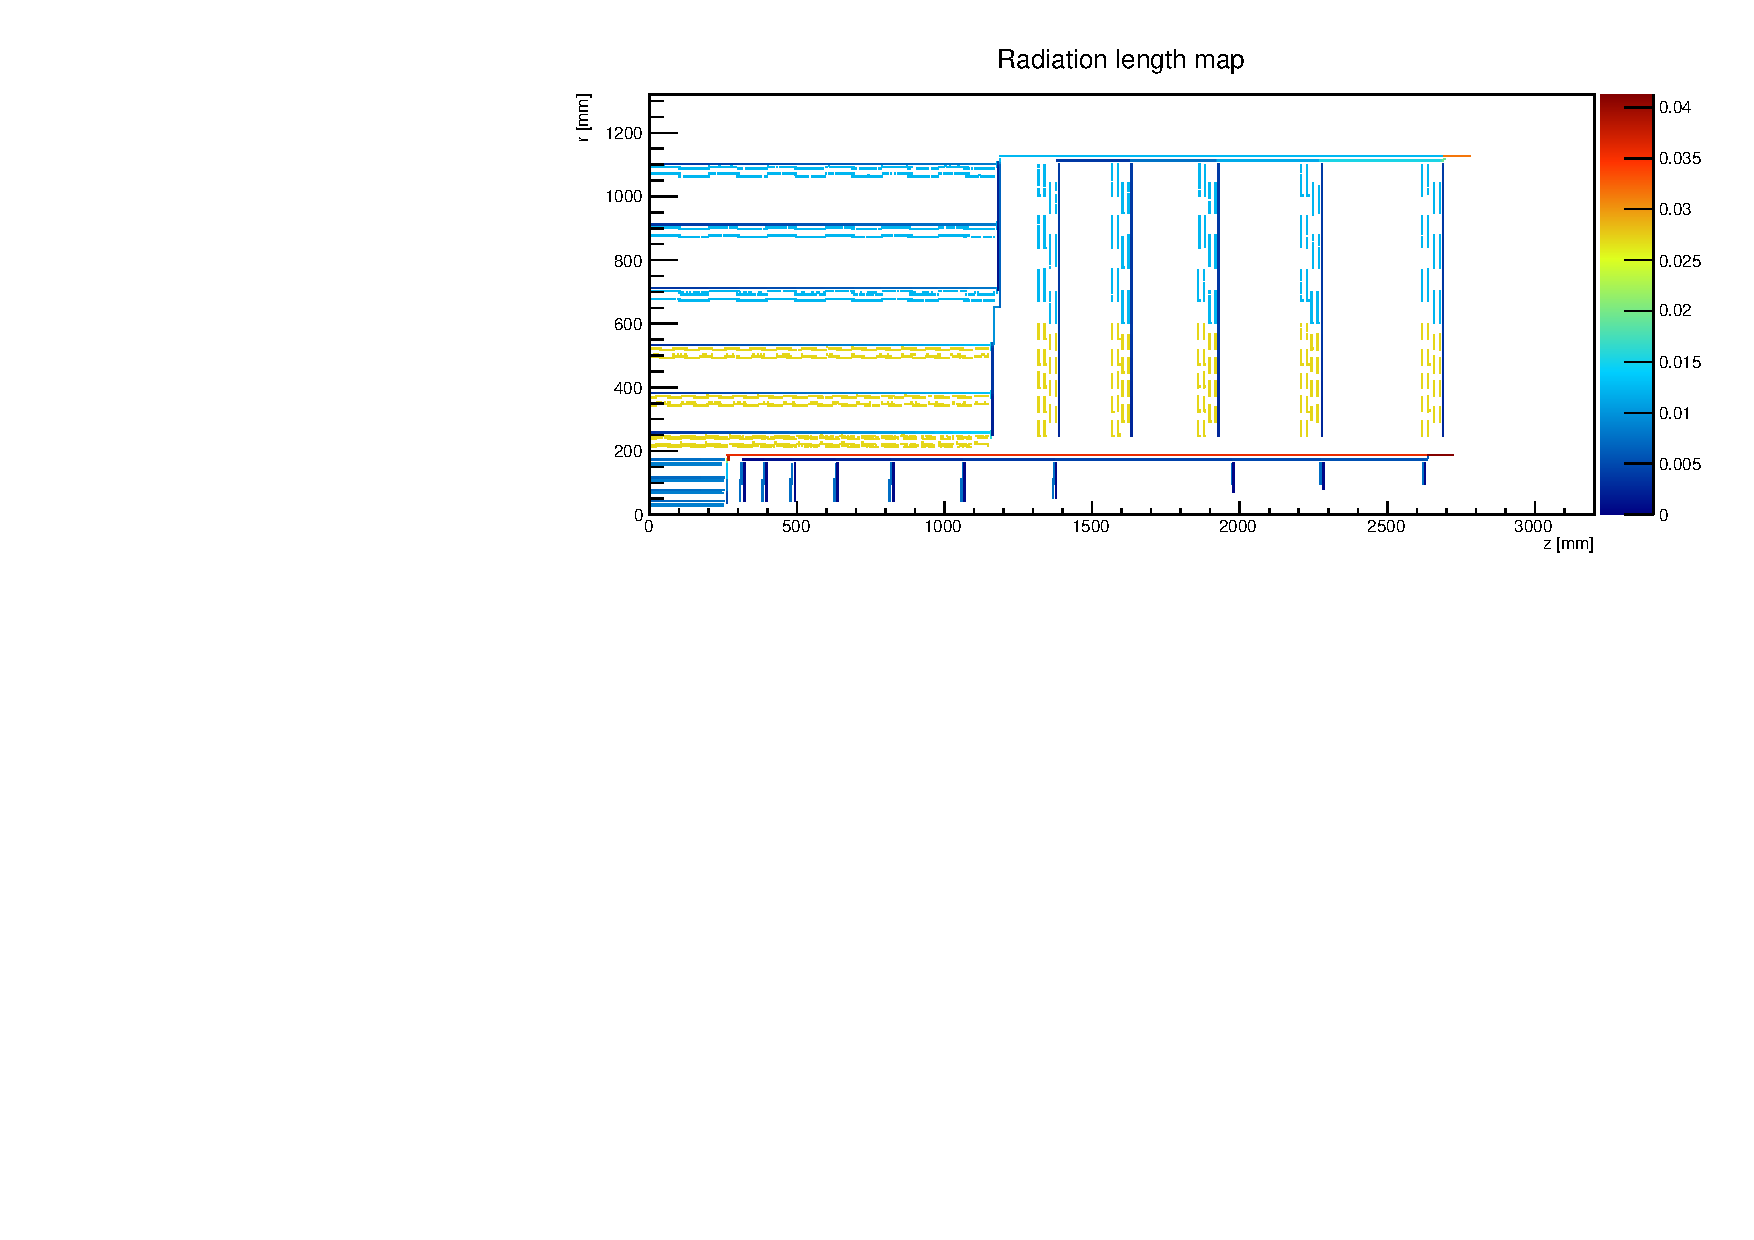
\includegraphics[width=\textwidth]{img/rad.pdf}
  \end{center}
\end{frame}

\begin{frame}{Rad./int. length Tech. prop., outer superimposition}
  \begin{center}
    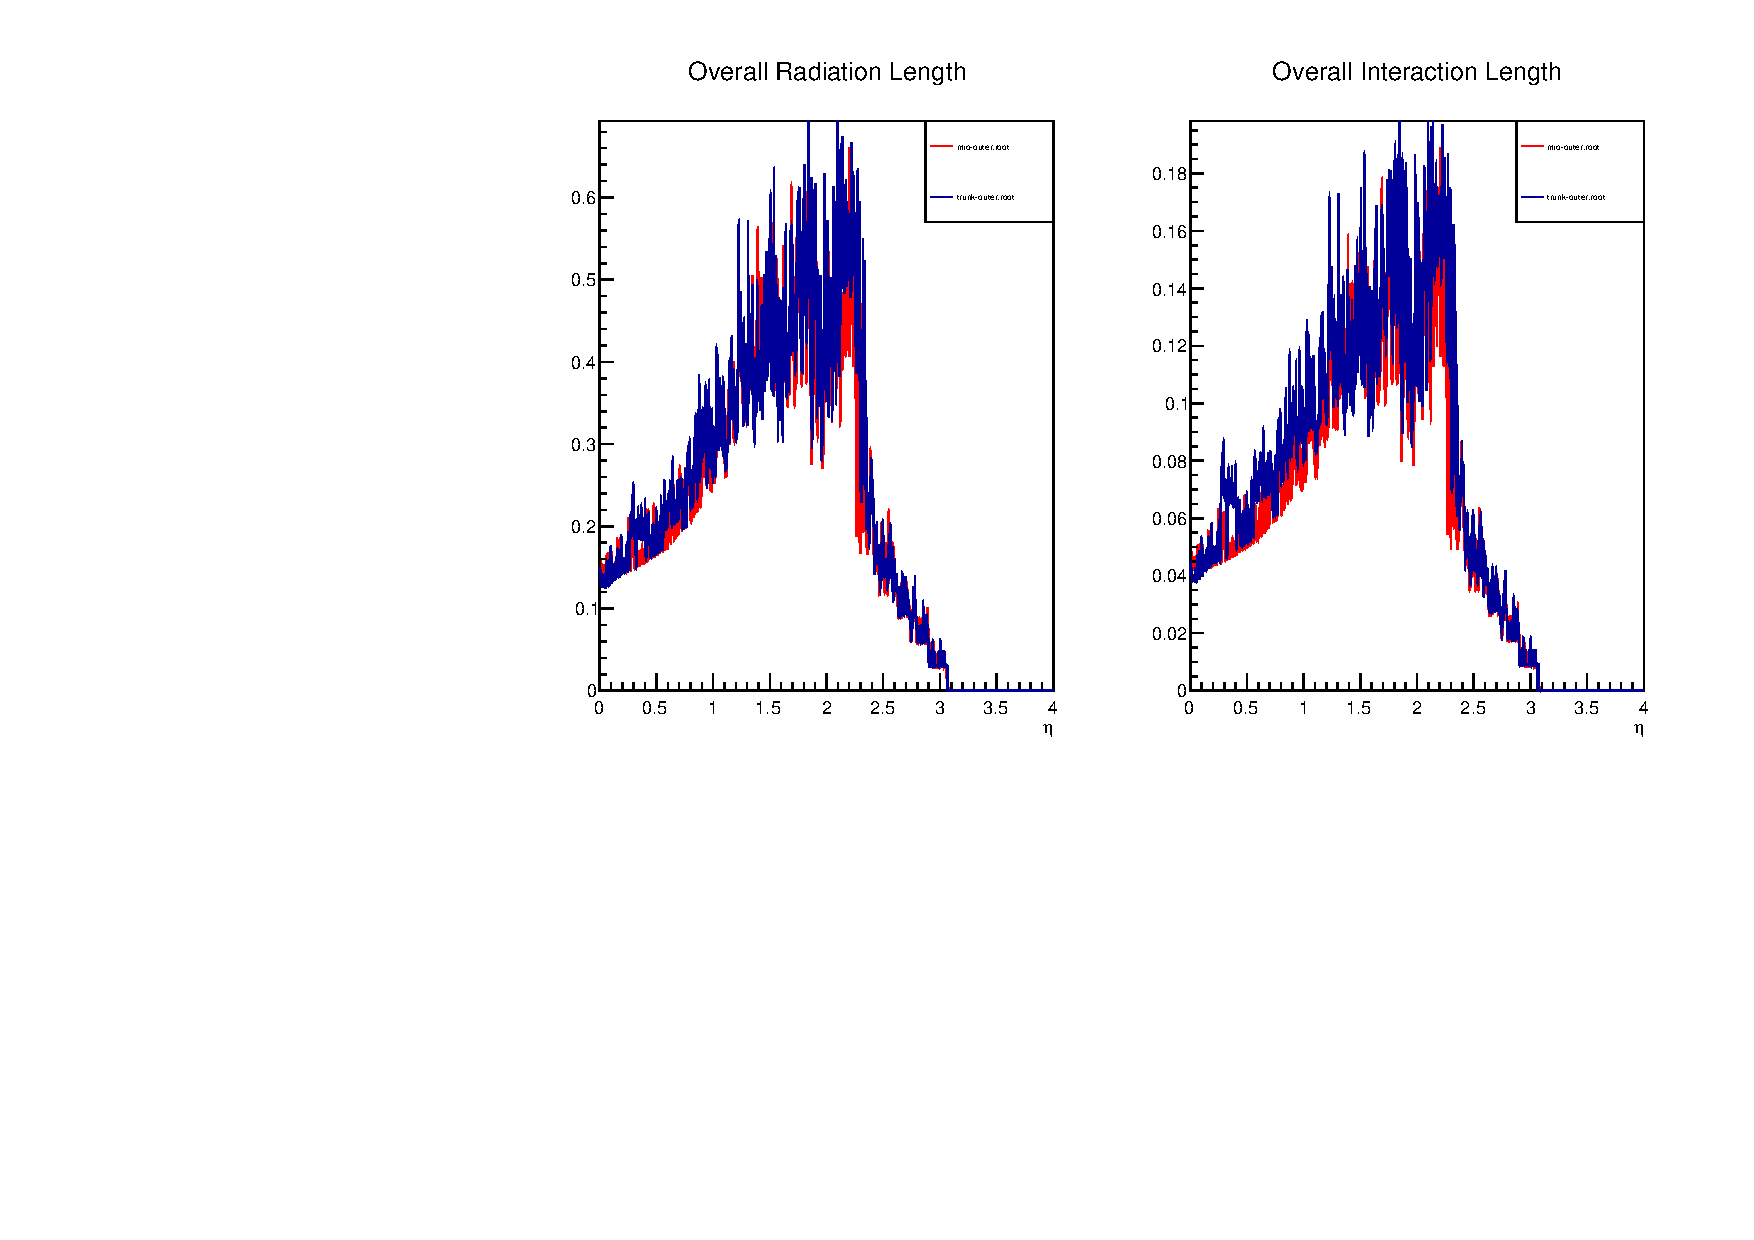
\includegraphics[width=\textwidth]{img/outer-superimposition.pdf}
  \end{center}
\end{frame}

\begin{frame}{Rad./int. length Tech. prop., outer scattering}
  \begin{center}
    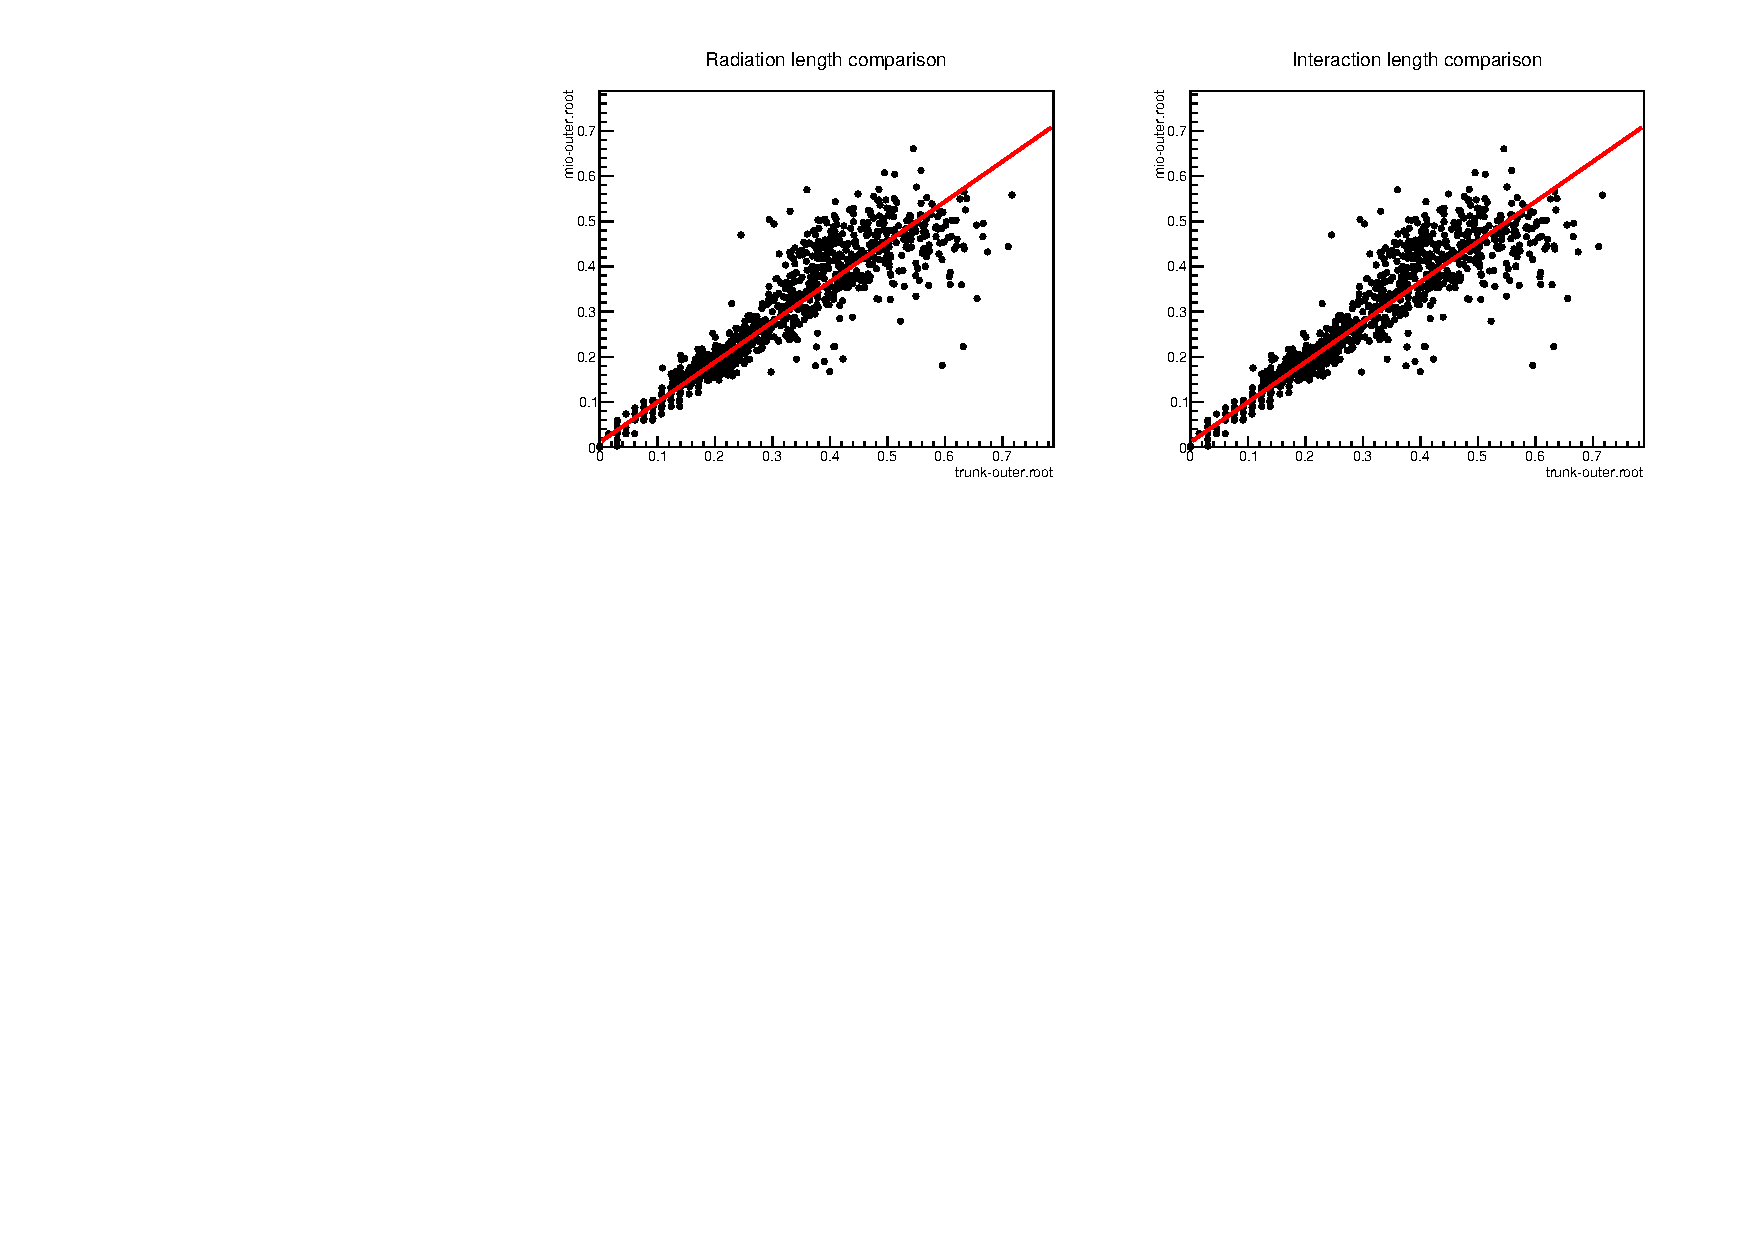
\includegraphics[width=\textwidth]{img/outer-scattering.pdf}
  \end{center}
\end{frame}

\begin{frame}{Rad./int. length Tech. prop., pixel superimposition}
  \begin{center}
    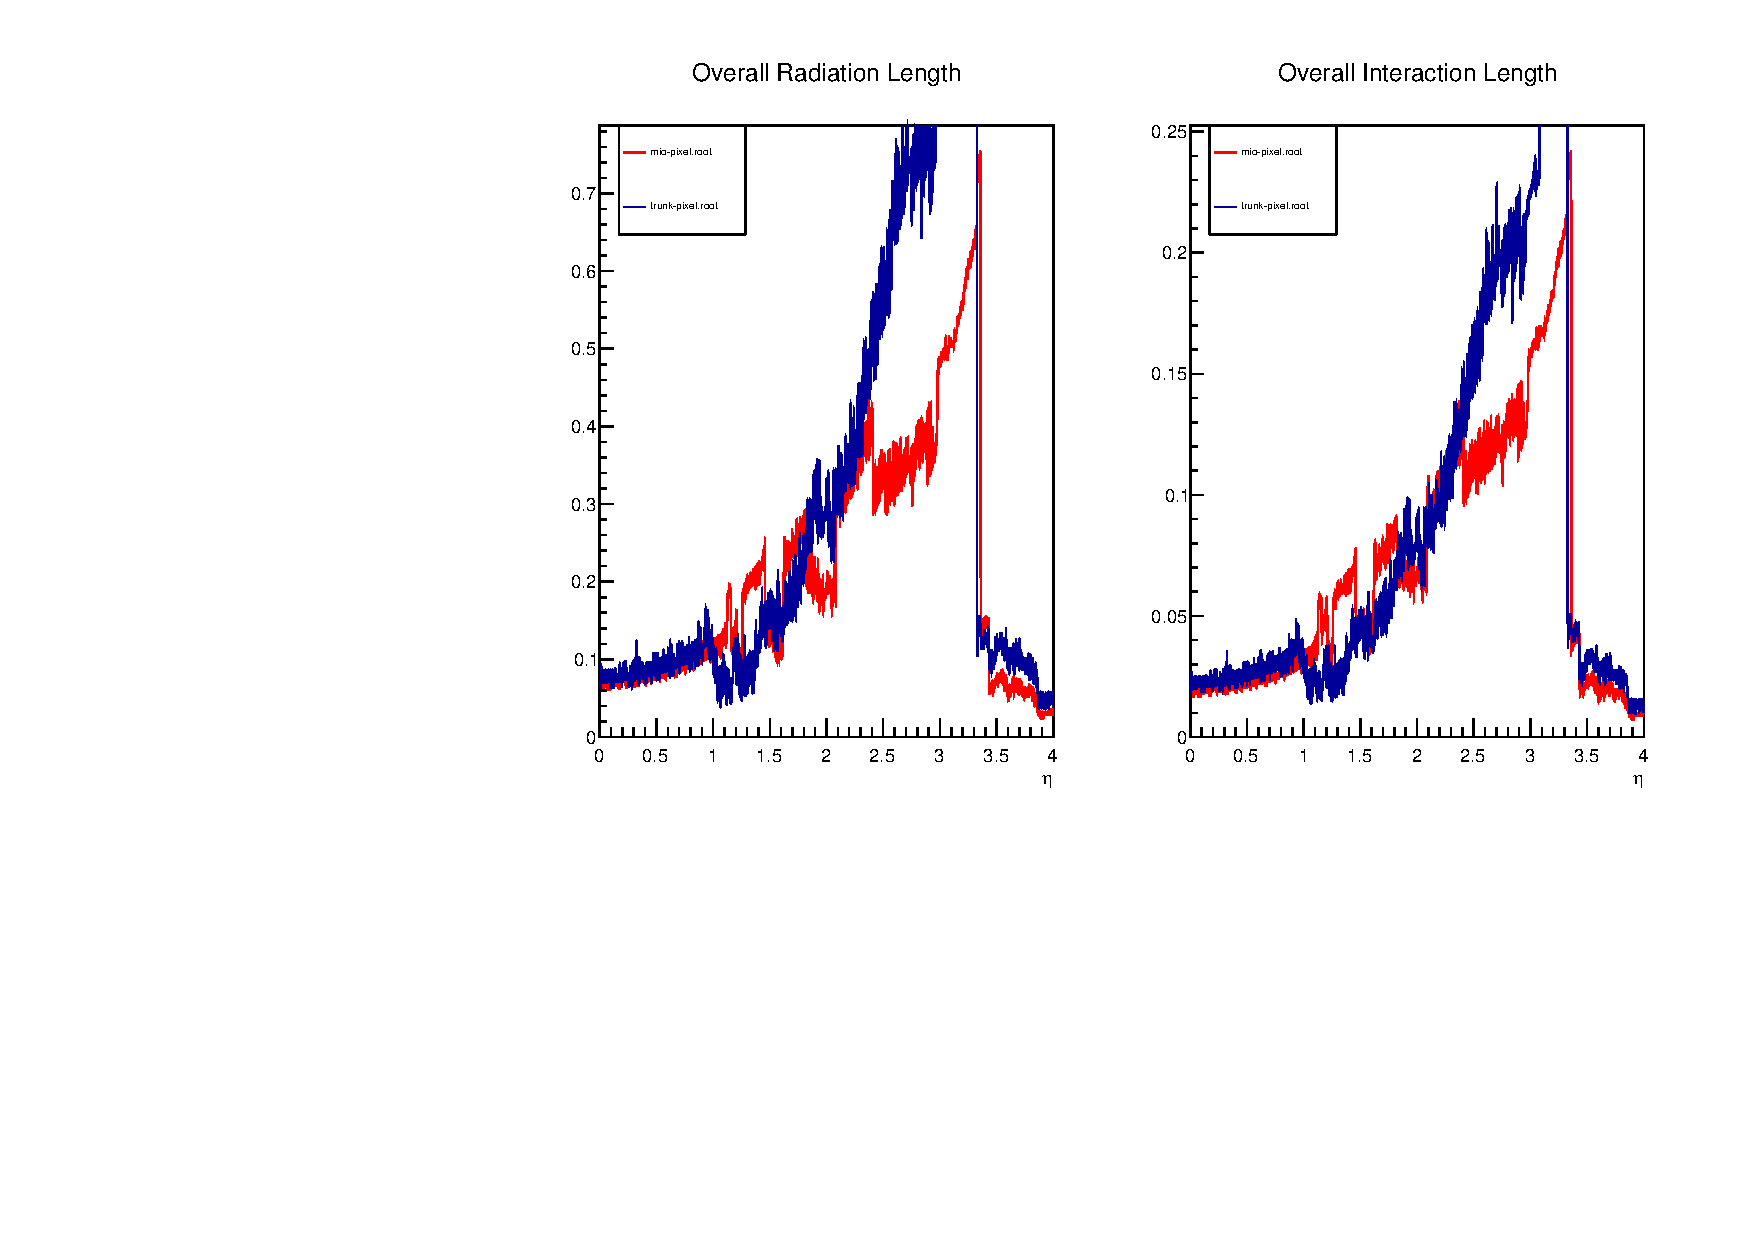
\includegraphics[width=\textwidth]{img/pixel-superimposition.pdf}
  \end{center}
\end{frame}

\begin{frame}{Rad./int. length Tech. prop., pixel scattering}
  \begin{center}
    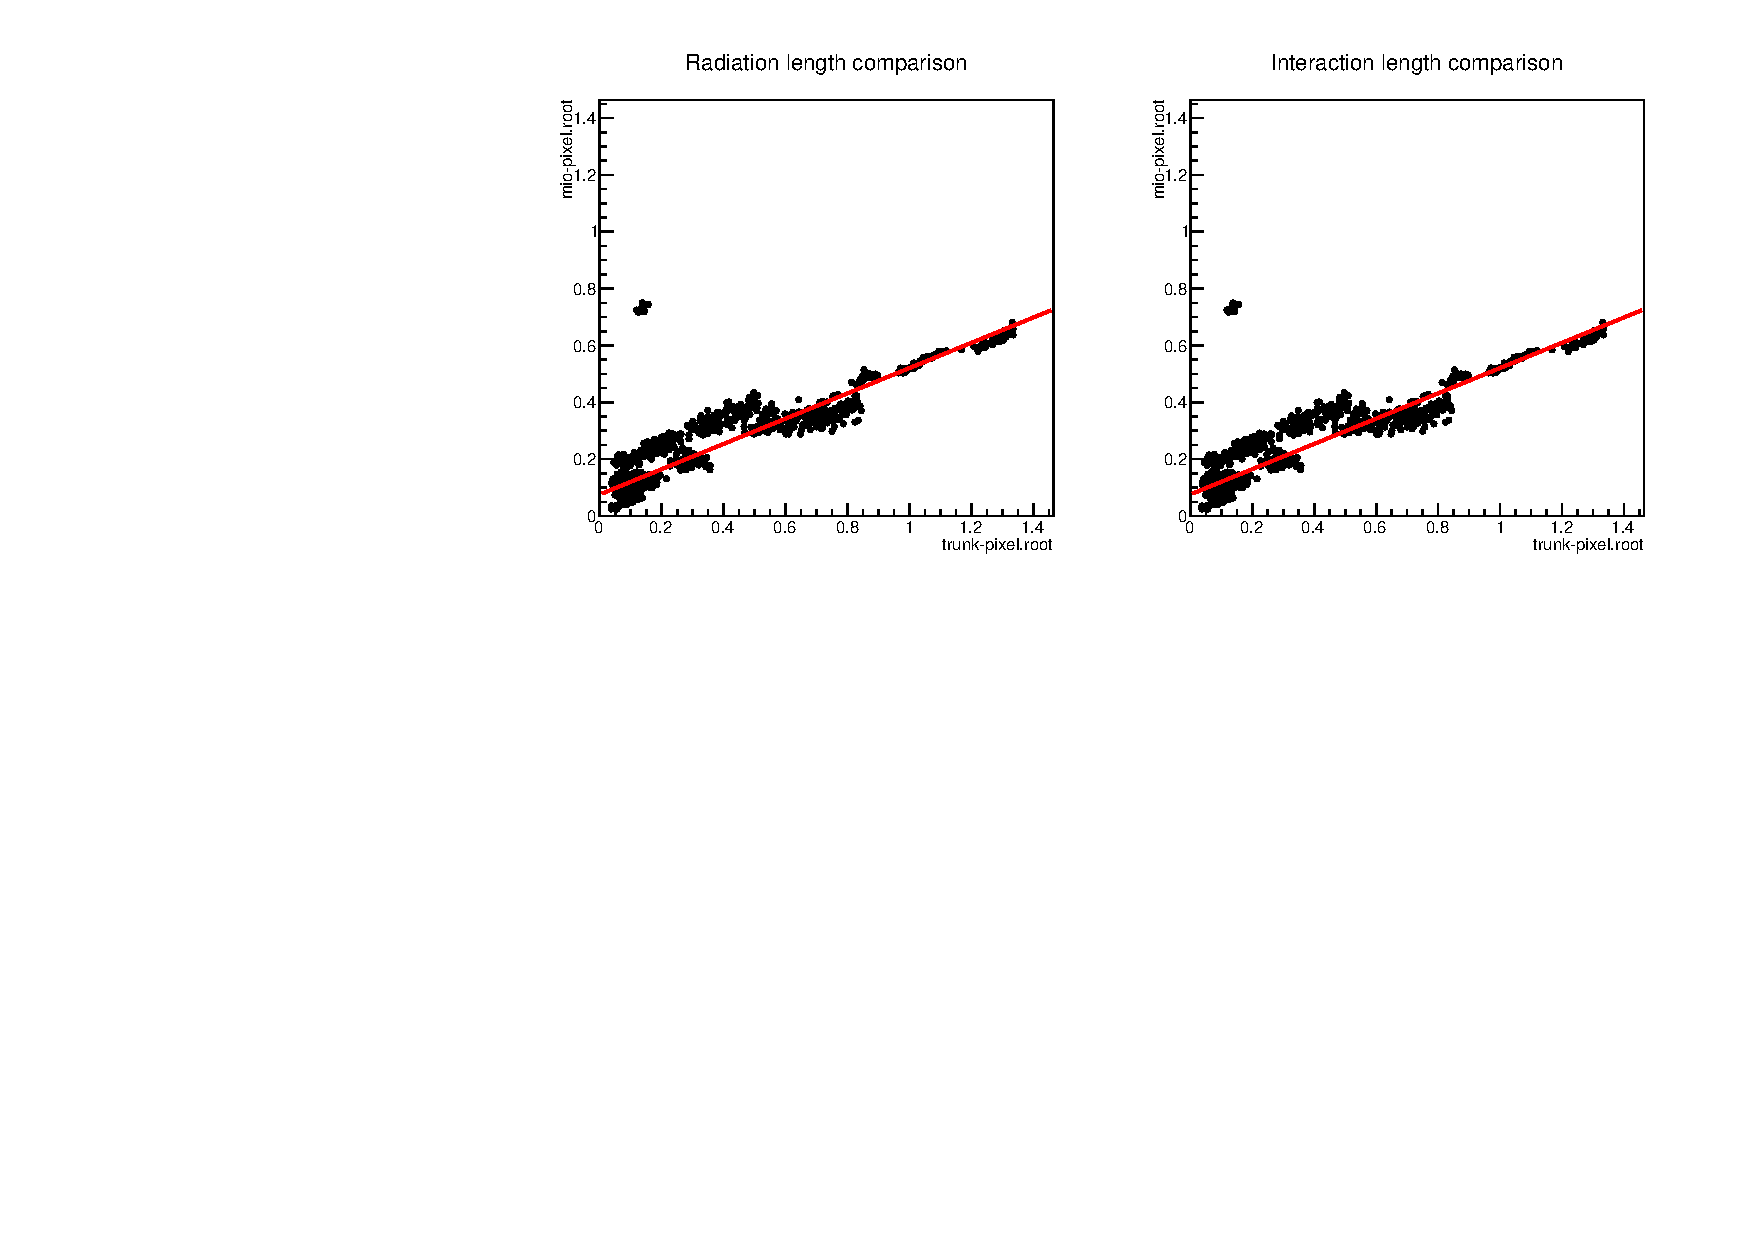
\includegraphics[width=\textwidth]{img/pixel-scattering.pdf}
  \end{center}
\end{frame}

\begin{frame}{Rad./int. length Tech. prop., pixel 2 superimposition}
  \begin{center}
    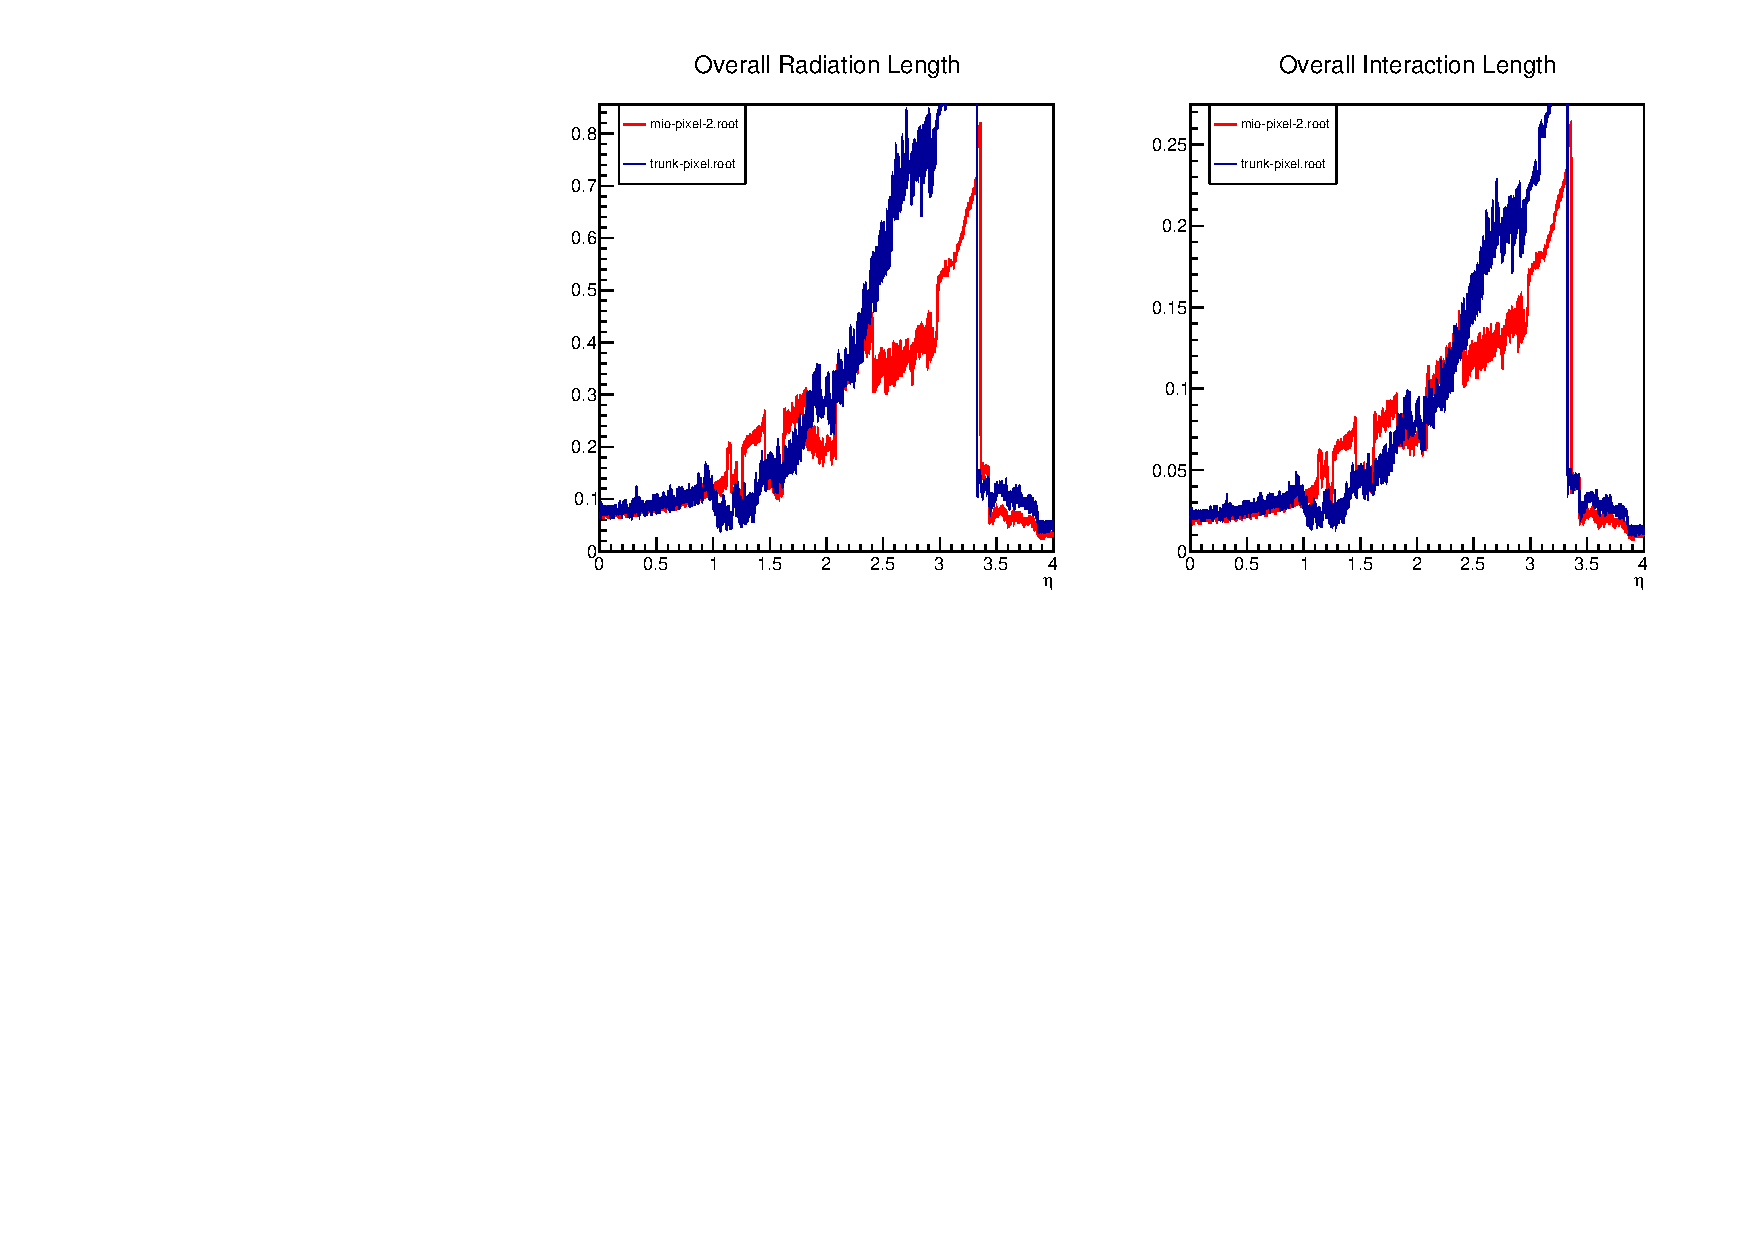
\includegraphics[width=\textwidth]{img/pixel-2-superimposition.pdf}
  \end{center}
\end{frame}

\begin{frame}{Rad./int. length Tech. prop., pixel 2 scattering}
  \begin{center}
    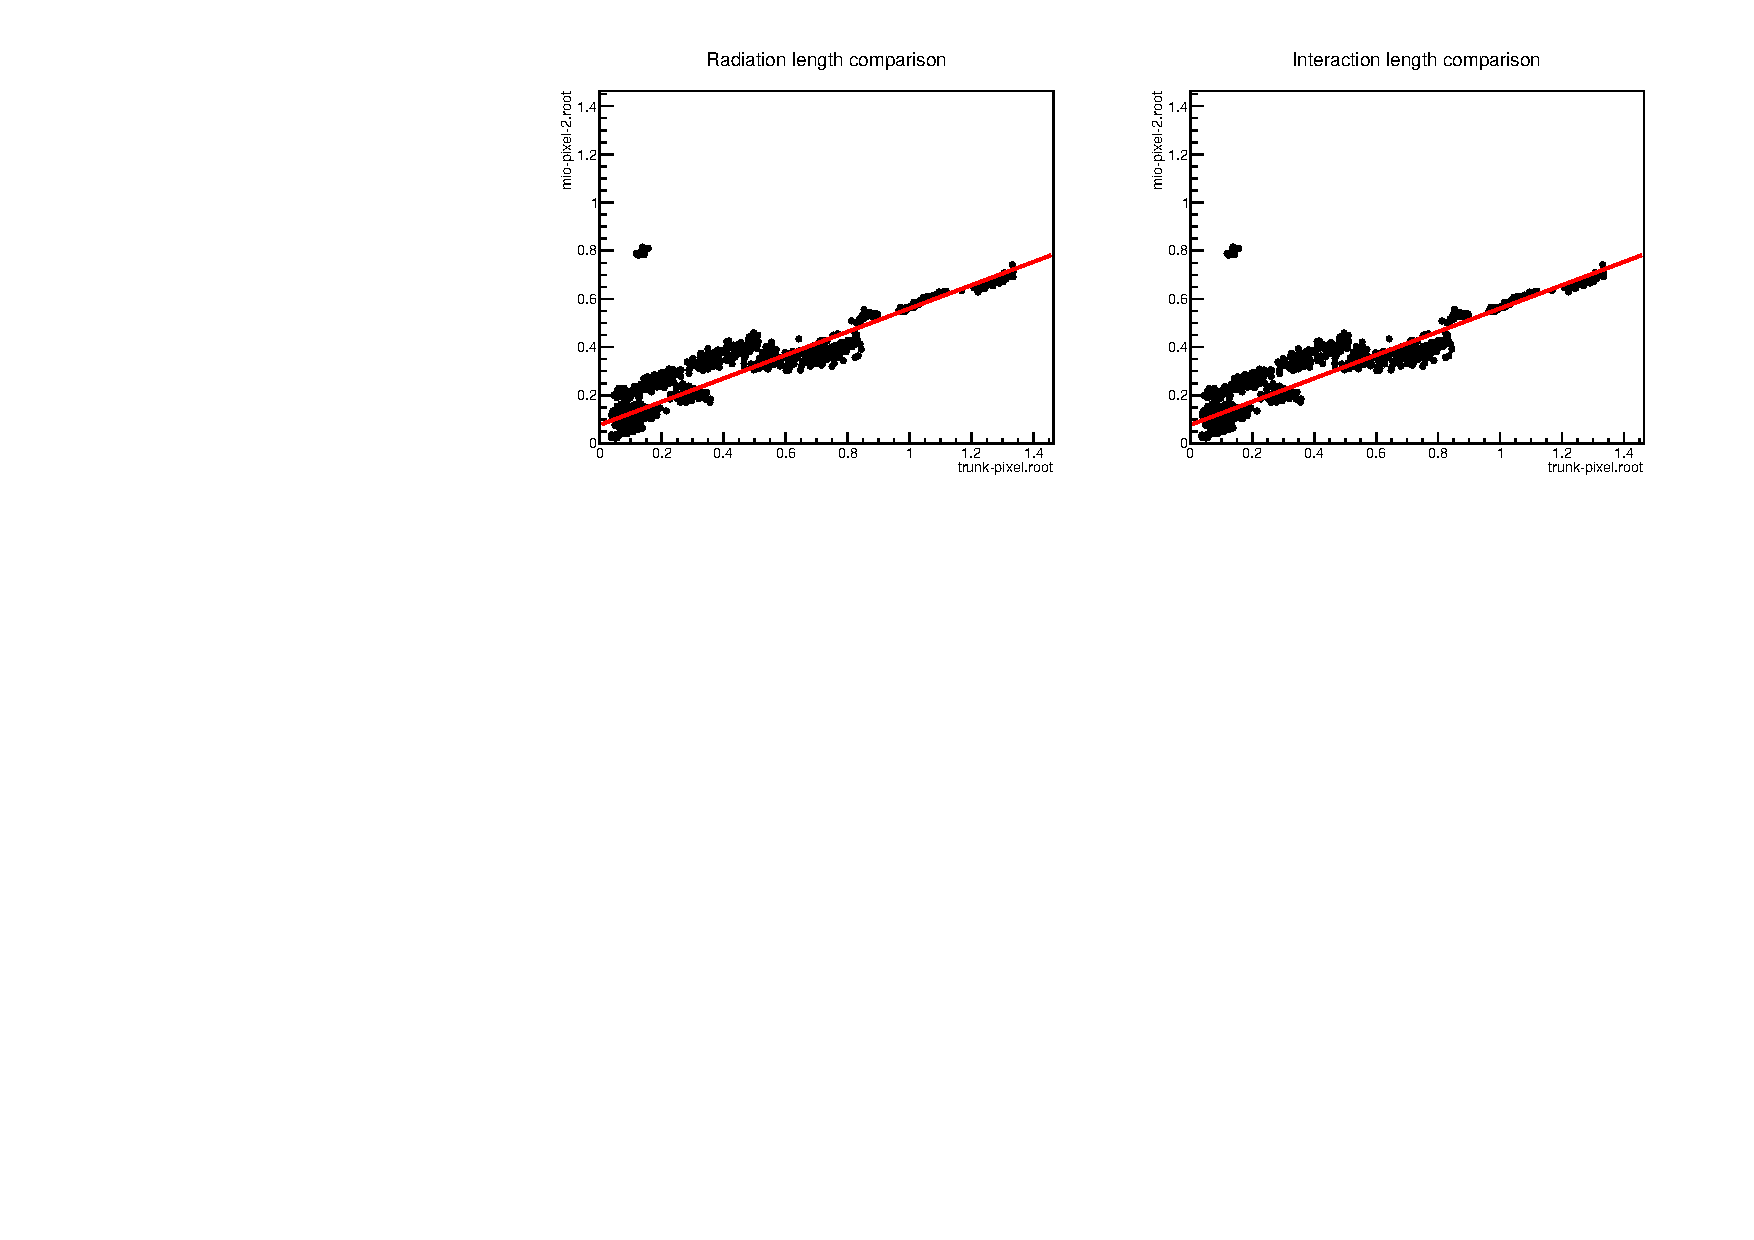
\includegraphics[width=\textwidth]{img/pixel-2-scattering.pdf}
  \end{center}
\end{frame}

\begin{frame}{Radiation length Tilted}
  \begin{center}
    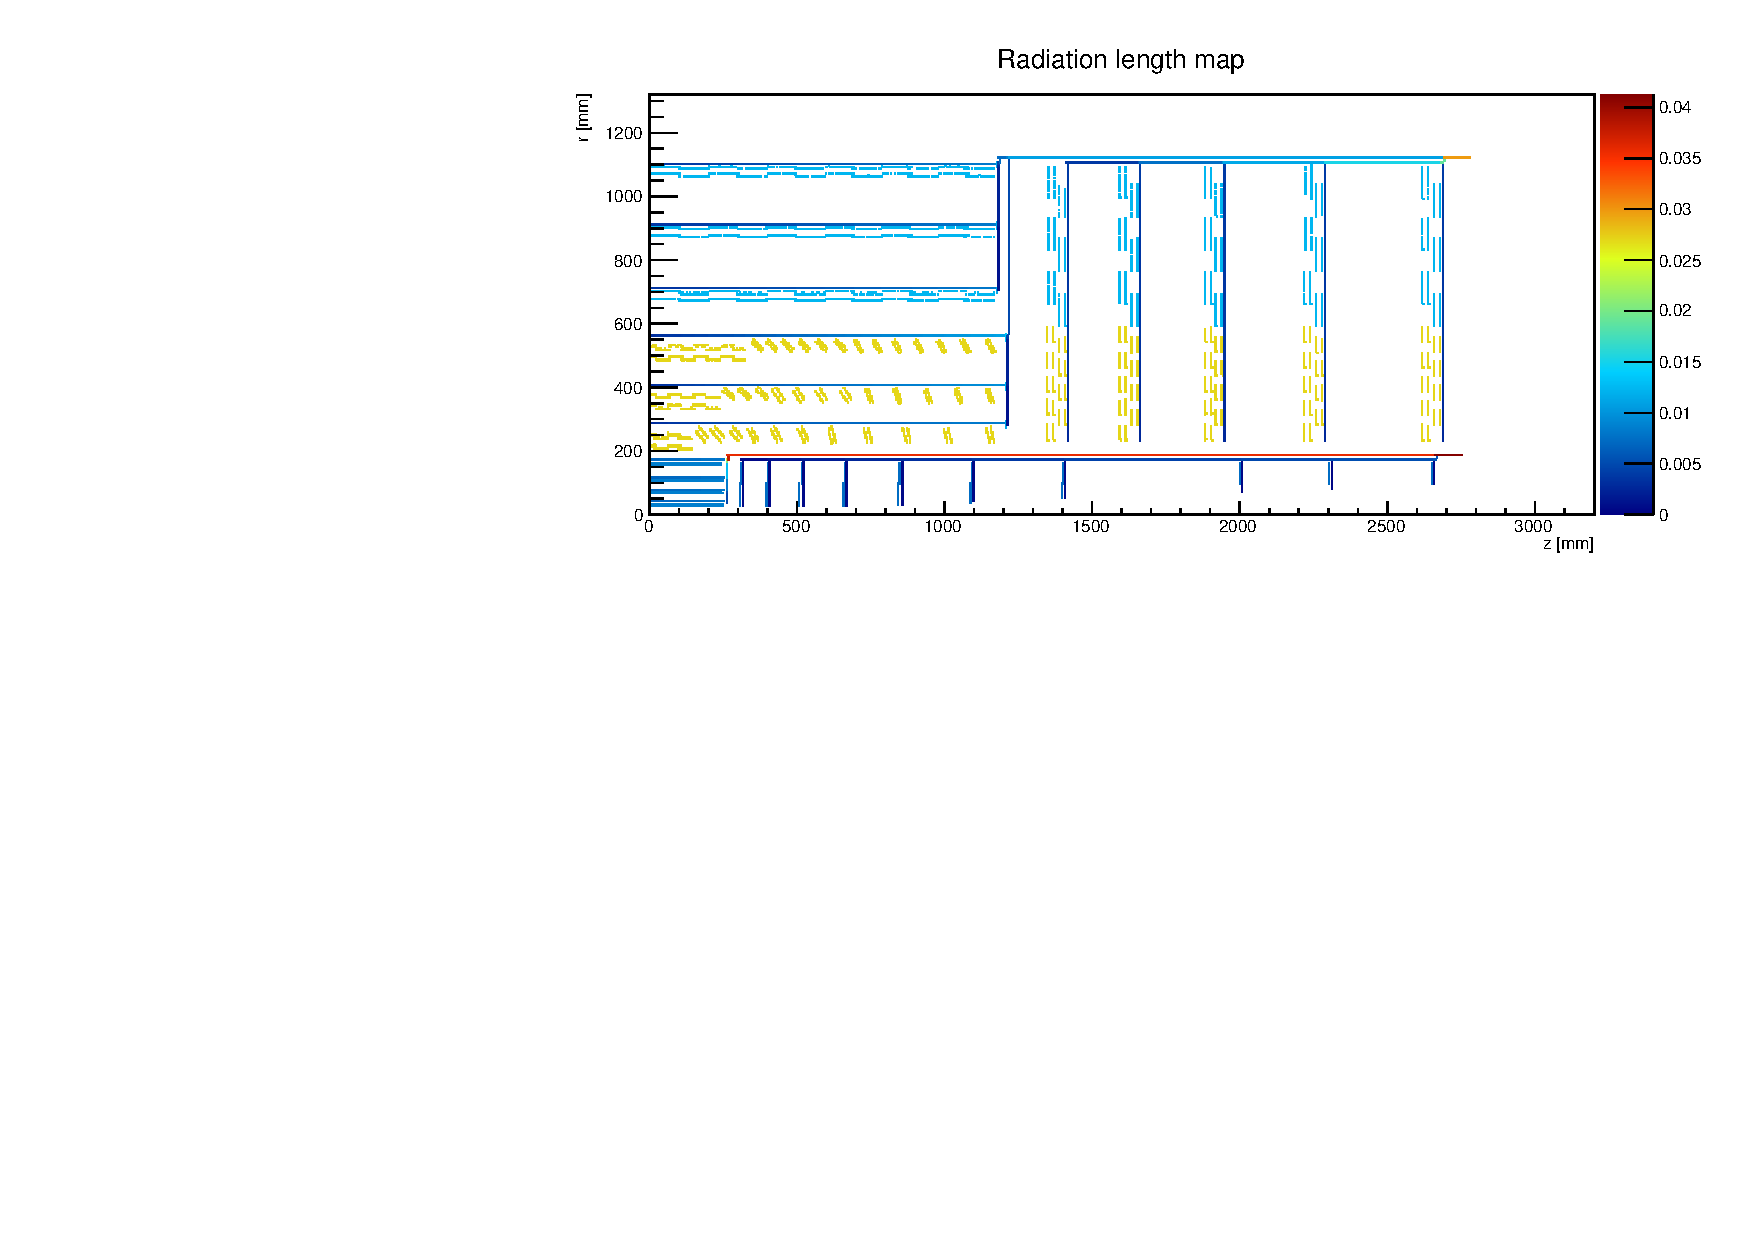
\includegraphics[width=\textwidth]{img/rad-tilted.pdf}
  \end{center}
\end{frame}

\begin{frame}{Rad./int. length Tilted, superimposition}
  \begin{center}
    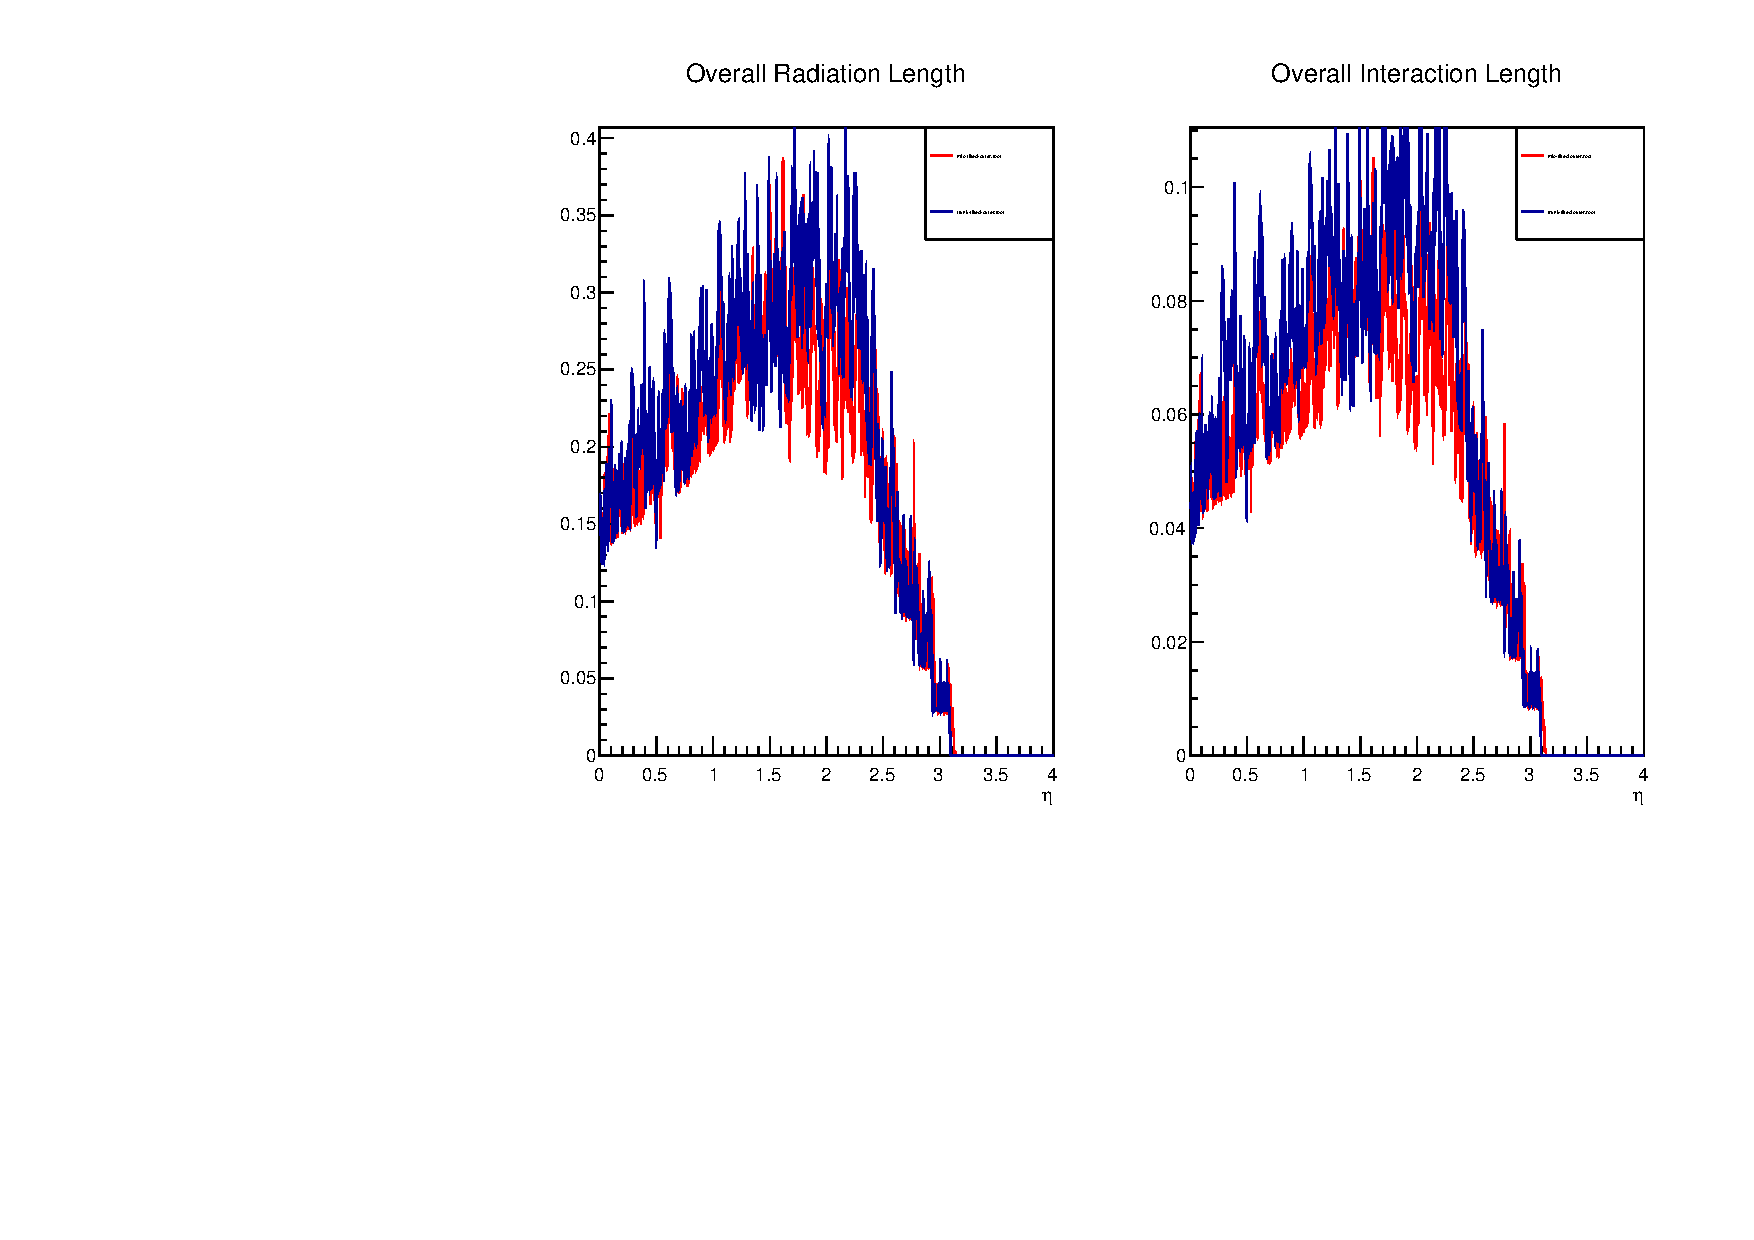
\includegraphics[width=\textwidth]{img/outer-tilted-superimposition.pdf}
  \end{center}
\end{frame}

\begin{frame}{Rad./int. length Tilted, superimposition}
  \begin{center}
    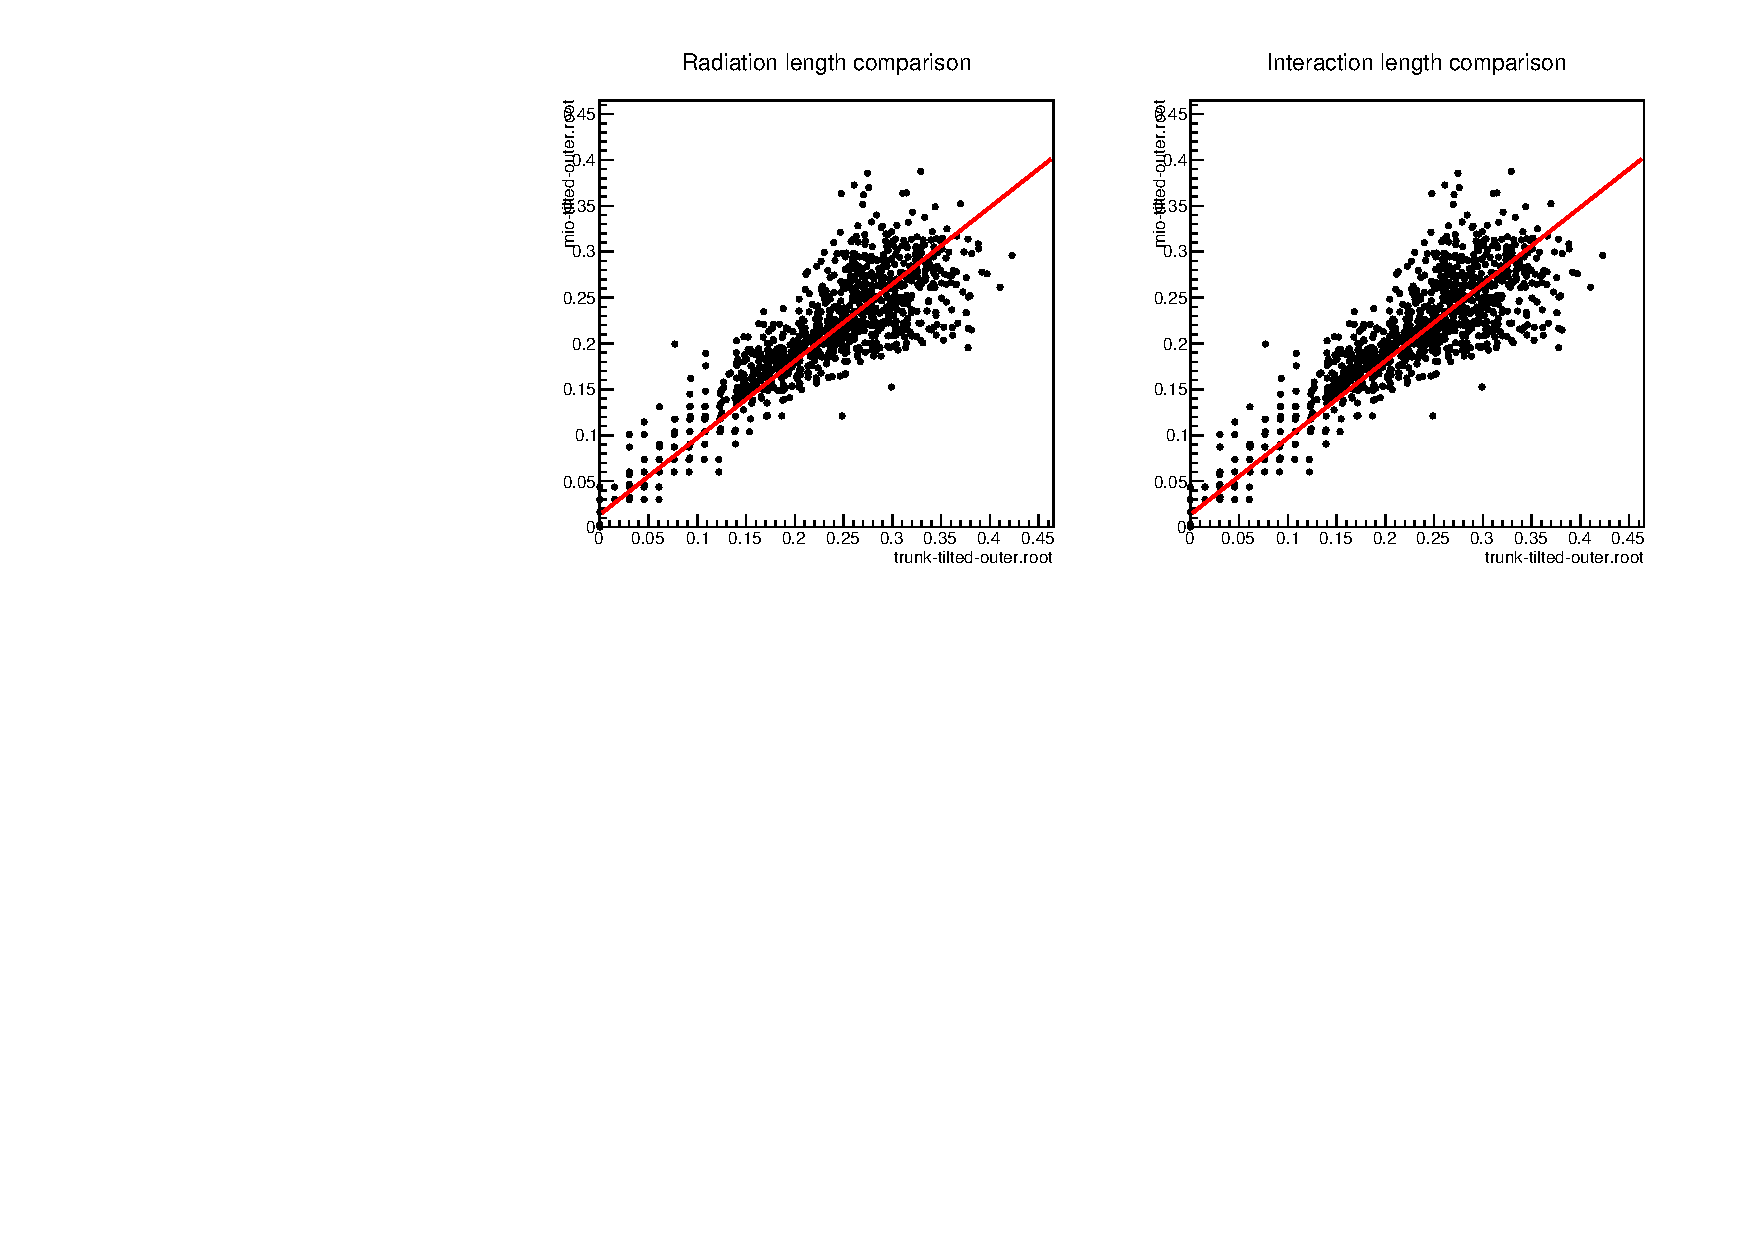
\includegraphics[width=\textwidth]{img/outer-tilted-scattering.pdf}
  \end{center}
\end{frame}

\begin{frame}{Second level station}
  \begin{center}
    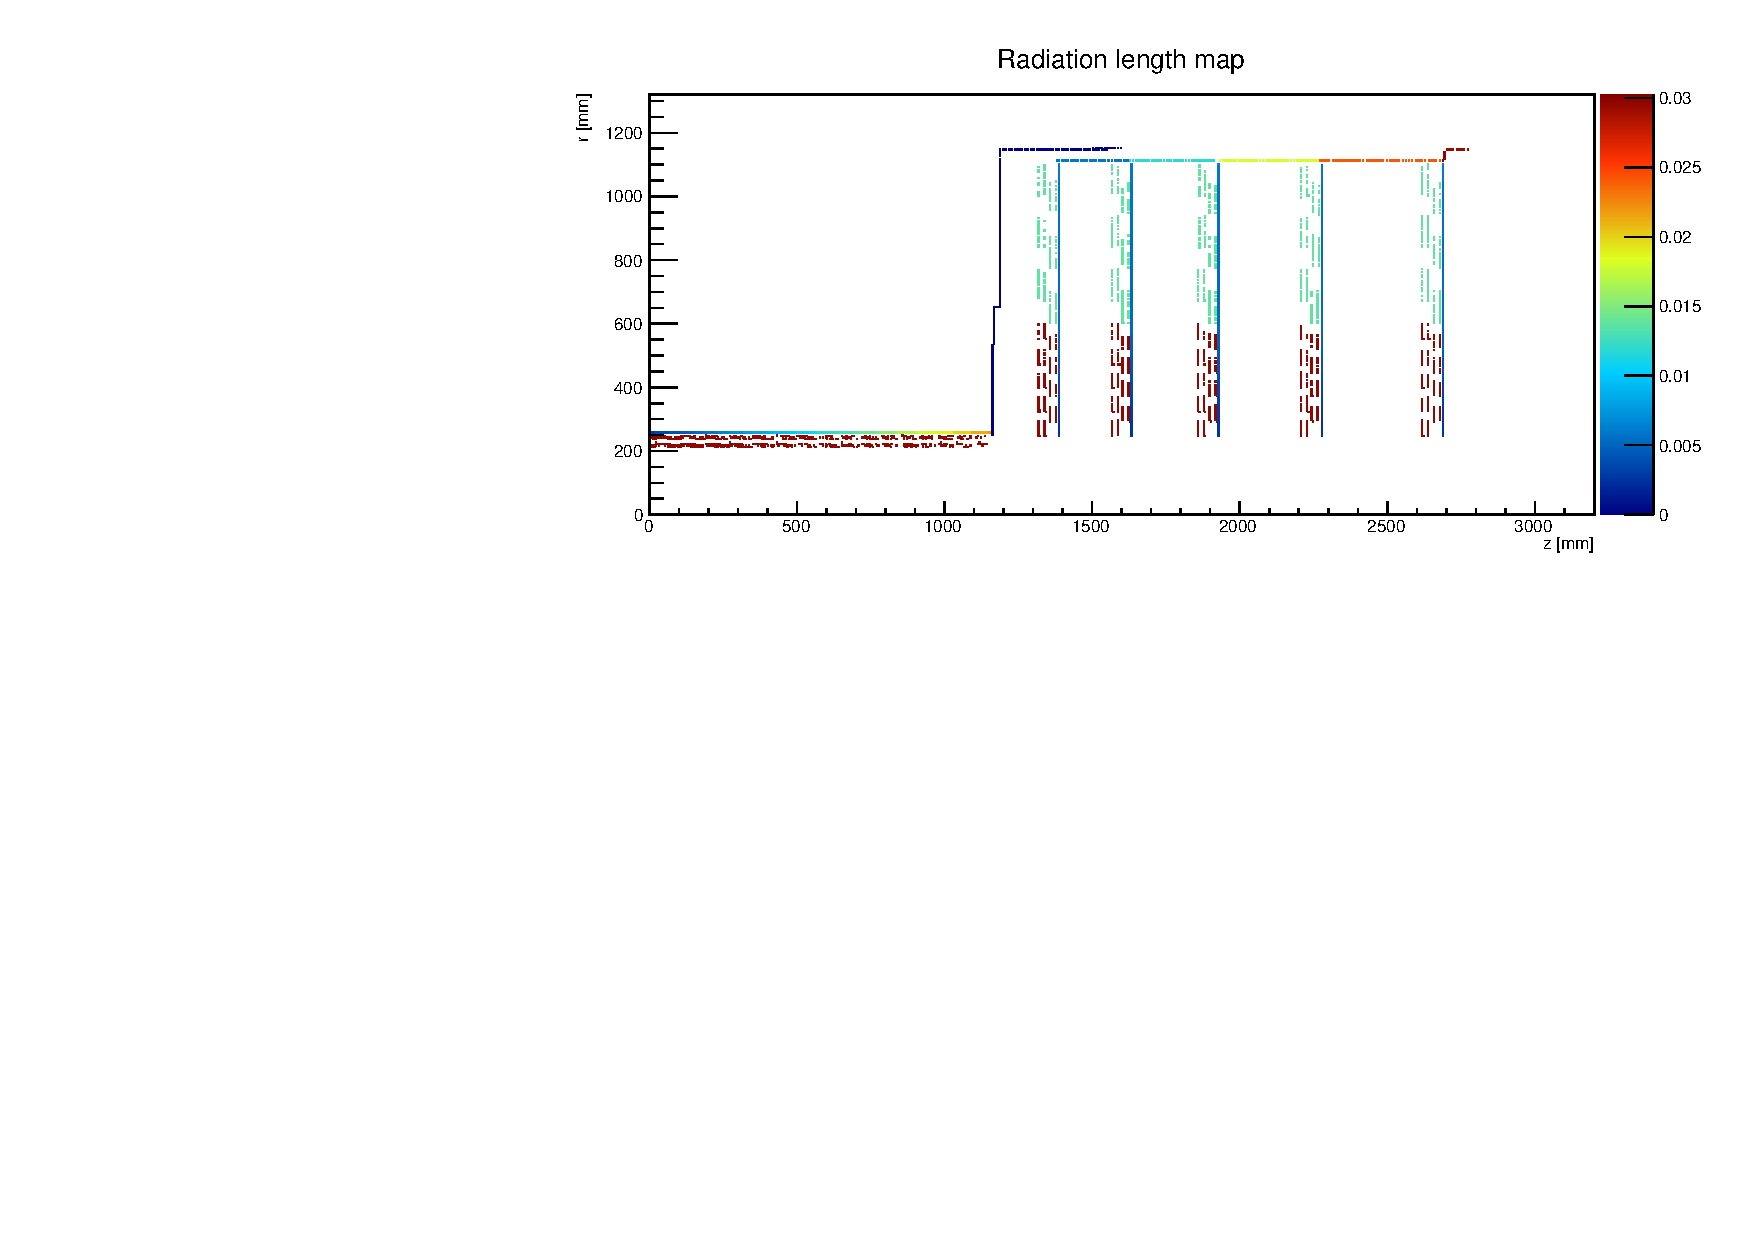
\includegraphics[width=\textwidth]{img/stazione2.pdf}
  \end{center}
\end{frame}

\begin{frame}
  \begin{block}{Done}
    \begin{itemize}
    \item Corrected scaling error
    \item Pixel materials
    \item Tested tilted
    \item Second level stations
    \end{itemize}
  \end{block}
  \begin{block}{To do}
    \begin{itemize}
    \item Adjust pixel config file?
    \item Support structure
    \end{itemize}
  \end{block}
\end{frame}

\end{document}
